% General comments / corrections:
% - be consistent in use of "B" vs "B molecules"
%
\section{Introduction}
\label{sec:Introduction}
% - carbon blacks instead of soot (materials focus)

%% Curved carbons are everywhere...
Curved carbons are found in many materials including porous carbons (ref), glassy carbons (ref), activated carbons (ref), carbon aerogels (ref), and soot particles~\cite{Martin2018flexo}. For example, high resolution transmission electron microscopy of energy-relevant carbon materials such as coal, coke, and soot, show that a significant proportion (28-49\% for mature carbons, 63\% for young particles) of the constituent molecules are curved \cite{wang2017improved,zhong2018structural,Martin2018flexo}. 
Curved carbons have many different names including bowl-shaped compounds, buckybowls, $\pi$-bowls, fullerene-like/fragments. In this work we will refer to them as curved polycyclic aromatic hydrocarbons (cPAHs), since flat polycyclic aromatic hydrocarbons (fPAHs) will be used as a comparison.

%% Curvature is caused by, properties 
What causes some carbon materials to be curved? Curvature is predominantly caused by the presence of non-hexagonal rings, such as pentagons, within a hexagonal lattice. The resulting molecules have steric and electronic properties not present in defect-free carbon materials containing hexagonal structures only. In particular, the curvature redistributes electronic charge in the $\pi$-cloud and causes the molecules to possess a dipole moment due to the flexoelectric effect \cite{Martin2017}. This allows curved molecules to interact in long-range electronic interactions, such as dipole-dipole interactions, not present in systems containing planar carbon molecules. However, these molecules retain aromaticity and show considerable electron delocalisation \cite{grabowsky2010electron}.

%% curved carbon applications...
These qualities cause the presence of curved aromatic molecules to influence material structure and properties. Curved molecules increase material porosity \cite{zhang2020molecular} and facilitate stronger adsorbate-adsorbent interactions \cite{demir2016adsorption}, which combined with high polarisability and high surface area provide enhanced adsorption important for applications such as carbon sequestration, gas storage and separation. Corannulene molecules, small aromatics containing a central pentagon, are often used as a model for microporous activated carbon \cite{demir2016adsorption,li2020molecular} used in such applications.

Curved aromatics also possess a combination of properties, including surface charge stabilisation, high charge mobility, significant dipole moment, fluorescence, and small band gap (refs), that make them excellent candidates for applications such as optoelectronic devices, organic semiconductors, liquid crystals, electrodes, imaging probes, and batteries (refs). For example, integrating corannulene inside insulating porous scaffolds allows electronic properties to be tuned and results in a 10,000-fold conductivity enhancement \cite{rice2018stack}. Flame-formed carbon nanoparticles show quantum dot behaviour \cite{liu2019flame}, which have shown great promise in bioimaging, photovoltaic and light emitting applications due to their biocompatibility, luminosity, and solubility \cite{zhang2012graphene}.
% Good promise in electronics applications because of tunable optoelectronic properties \cite{sanyal2014functional}
% suggested for sensors and molecular machines (10.1039/c6cp05841h)

The alignment of columnar or stacked structures is important for mechanical and electronic properties of materials, and for the generation of graphisiting material. In some cases the presence of curved molecules contributes to a low degree of molecular ordering in a material %and poor stacking (only ~20\% stacked)
\cite{zhong2018structural} and may prevent graphitisation by disrupting the formation of the mesophase. For example, the integration of curvature in molecules is crucial in determining whether a carbonised material produces graphitic or non-graphitised carbon \cite{abrahamson2018carbon}. Columns of cPAHs also show high electron transport characteristics desirable for high-performance materials for organic electron devices \cite{wang2015electronic}.

Accurately describing and characterising the structure and self-assembly of curved carbon materials is of interest to production processes since curvature is easily integrated as a defect (more stable than planar). This is crucial for understanding many ubiquitous materials, such as combustion-produced particles and graphite from mesophase pitch.
%
%Carbon materials have been fabricated for use as adsorbents, carriers, catalyst supports, electrodes, and other advanced applications (refs).  The performance of these materials can be directly improved/tuned for these applications by adjusting their physical properties - in particular their nanostructures.  It is therefore crucial to develop a detailed understanding of the molecular interactions involved to enhance the prediction and design of desired carbon nanostructures.

%% Arrangement of atoms determines everything...
The arrangement of atoms in a carbon material determines its structure, properties, and function. Nanostructure is crucial to understand the existing and potential behaviour of carbon materials. For example, it provides the understanding of (how to optimise) a structure's stability/longevity, environmental interactions, and ability to store other molecules, which are all vital for gas storage, drug delivery, or sequestration applications.  Similar information about the detailed structure of the material is required for other applications such as batteries, adsorbents, sensors, and novel nanocarbon materials.
In addition to providing the understanding required to optimise the nanostructures for these applications, this provides insight into the natural processes and environments that generate nanoparticles containing polycyclic aromatic hydrocarbons, such as combustion-produced pollutants (ref) and interstellar medium (ref).

%% Previous work looking at cPAH interactions:	Homogeneous dimers; Pi-pi > pi-CH interactions, eclipsed > staggered.
Previous work on the structure and properties of polycyclic aromatic hydrocarbons has focused on those that are flat/planar (fPAHs) \cite{Grancic2016,chen2014size,Rapacioli2005stacked,hernandez2017dynamics}, with less attention given to curved PAHs (cPAHs). Electronic structure calculations show that there is significant energy in interactions between nested concave-to-convex homogeneous cPAH dimers, and their curvature does not prevent dimers from forming $\pi$-$\pi$ stacked assemblies similar to planar systems \cite{sygula2009pi,Cabaleiro-Lago2018}. As with fPAHs, cPAH dimer interactions are dominated by $\pi$-$\pi$ interactions compared to CH-$\pi$ interactions. However cPAHs in the concave-convex dimer configuration show different behaviour than fPAH dimers and cPAHs in convex-convex configuration, with the eclipsed dimer (in which the aromatic planes are aligned) showing a higher stability than the staggered dimer (in which the aromatic planes are shifted relative to each other) \cite{janowski2011convex,Cabaleiro-Lago2018}.
Dispersion provides the dominant energy contribution, although electrostatics are also significant especially in contrast to fPAH dimers (\cite{Cabaleiro-Lago2018,janowski2011convex}.

Different degrees of curvature can result in increased or decreased cPAH dimer strengths, due to geometry and (less so) electrostatic effects. Curvature is able to increase interaction strength by decreasing C-C distances for increased dispersion interactions \cite{kennedy2012buckyplates}. 
%However, very curved PAHs have lower interaction strengths similar to fPAHs due to increased steric hinderance (10.1016/j.proci.2018.05.046, \cite{sygula2009pi}). High curvature also increases exchange-repulsion and can destabilise the dimer (\cite{kennedy2012buckyplates}, \cite{sygula2009pi}).

%% Previous work looking at cPAH interactions:	Bulk systems
X-ray and density functional theory calculations have shown that the crystal structure of cPAH systems are determined by an interplay of electrostatic and dispersive forces, but predicting the packed structure of cPAHs is not obvious. The dipole moment and molecule bowl depth are identified as significant factors, but do not have clear threshold values that guarantee particular molecular arrangements \cite{Filatov2010}. In addition, the size, curvature, rigidity, functionalisation, and atomic composition of cPAHs are known to influence their ability to form columnar stacks in solid state \cite{wang2015electronic,scott1999geodesic,grabowsky2010electron,sygula1994bowl,bronstein2002practical,forkey1997crystallographic,roch2017indenocorannulene,petrukhina2004hemibuckminsterfullerene,petrukhina2005unprecedented,Filatov2010,sakurai2005structural,imamura1999triphenyleno,wu2006aromatic,sanyal2014functional}. These systems show large $\pi$-$\pi$ overlap and staggered stacked interactions to produce extended $\pi$ networks enhanced by CH-$\pi$ interactions.

%% Previous work looking at cPAH interactions:	Heterogeneous systems (dimers, etc)
% need to do a better job at splitting ideas: increased electrostatics and interactions with ions vs different structure and bowl complementarity
Computational studies of fPAHs show that, unlike cPAHs, heterogeneous dimers are significantly weaker than their homogeneous counterparts (ref). This heterogeneity was shown to decrease the stability of a nanoparticle containing different molecule sizes and lead to a distinct partitioning in which the larger molecules formed the cluster core and the smaller molecules resided in the outer shell \cite{bowal2018partitioning}. Dynamic interactions of cPAHs or fPAHs with cations also highlighted the ability of cPAHs to engage in electrostatic interactions that stabilise a cPAH cluster, while fPAHs cannot \cite{bowal2019ion}. These results suggest that the fundamental interaction differences between fPAHs and cPAHs may cause different clustering and packing behaviours. Preliminary work suggests that the nanostructure of homogeneous cPAH clusters is significantly different from similar-sized fPAH clusters \cite{bowal2019ion}, and perhaps different molecule sizes will show increased packing and stability due to bowl complementarity.
% This may be more representative of the experimentally observed structure of nascent soot particles.

%So expect homogeneous corannulene nanocluster to be disordered, homo 2pent15ring cluster to have stacks. Expect mixed cPAH cluster to be dominated by 2pent15rings but enhanced corannulene stacking and more stable than comparable mixed fPAH cluster.
% cPAH interactions with different sized molecules (no heteroatoms) (refs????). Increased stability compared to heterogeneous fPAH systems because of shape fitting and enhanced electrostatics and CH-pi interactions (?).
%Homodimers are weaker than heterodimers because they don't take advantage of bowl complementarity (\cite{Cabaleiro-Lago2018}).
%Thus we hypothesise that heterogeneous cPAH clusters may be more stable than their heterogeneous fPAH counterparts since different sizes of cPAHs may provide stable packing arrangements.
%

%% Limitations of existing work
To date, detailed studies of cPAHs have primarily included static DFT calculations or crystal structure experiments, as described above, neither of which provide information about intermolecular dynamics and particle nanostructure.
%
%% purpose of this work... 
%The structural properties of cPAH clusters are unknown and further molecular modelling studies are required to provide insight into the clustering behaviour of cPAHs - their size-dependent arrangements in both homogeneous and heterogeneous systems, interactions with planar PAHs, and assembly around ions. Understanding non-covalent interactions with and between curved carbon nanostructures has importance in many systems and great potential for numerous applications.
% Development requires understanding of self-assembly and dynamic nanostructure of curved aromatics
%
The purpose of this work is to explore properties of clusters containing curved PAHs, with the aim of answer the following questions: What is the energy and structure of cPAH nanoparticle systems and how do these differ from systems containing fPAHs? What is the influence of molecule size, proportion, and presence of ions or fPAHs?
%with the aim of answering the following questions: Are cPAH clusters more stable than fPAH clusters? Do cPAHs partition within clusters the same way fPAHs do? What is the internal nanostructure and surface composition of cPAH particles?  
%Predict long-range dipole-dipole interactions increase stability.
%In this work, we are motivated to understand the influence of cPAHs in soot particle structure and stability, but these results have general relevance to nanoparticles containing cPAHs regardless of source or application.
%Hypothesis: cPAH clusters are more representative of the experimentally observed structure of nascent soot particles, heterogeneous cPAH clusters are significant since they are stable than their fPAH counterparts.
This is important for better understanding carbon nanomaterial applications such as batteries, imaging probes, gas storage, optoelectronics, and targeted nanomedicine.
We address these questions by studying nanoparticle systems containing cPAHs, first in homogeneous clusters containing one molecule type only, then extending this to heterogeneous clusters to understand the interactions and effect of cPAH size and ratio. Finally, exploratory work on systems containing cations and fPAHs is presented.

%%%%%%%%%%%%%% Other notes to perhaps include %%%%%%%%%%%%%
% Functionalisation allows stacking solid-state structure in corannulene systems (chemical nature and position of functional groups strongly affects the stacking geometry) which influence optoelectronic properties \cite{sanyal2014functional,mack2007development}.
% "Properties of a matter are intrinsically dependent on the internal arrangement of molecules in the solid state. Therefore, knowledge of three-dimensional structure of the matter is a prerequisite for structure–property correlations and design of functional materials. Over the past century, X-ray crystallography has evolved as a method of choice for accurate determination of molecular structure at atomic resolution. The structural information obtained from crystallographic analysis paved the way for rapid development in electronic devices, mineralogy, geosciences, materials science, pharmaceuticals, etc."


\section{Methods}
\subsection{Systems} %% systems studied
To thoroughly evaluate the self-assembly of nanoparticles containing cPAHs, %influence of particle size, molecule size, molecule ratio, and ion interactions, 
16 different clusters are evaluated. Three different molecule types with different sizes and degrees of curvature are considered: coronene (\ce{C24H12}), a small fPAH containing seven hexagons, corannulene (\ce{C20H10}), the smallest cPAH containing one central pentagon with five surrounding hexagonal rings, and \ce{C42H14}, a larger cPAH containing two embedded pentagons. The two cPAHs are shown in Figure~\ref{fig:clustersnapshots}.
First, homogeneous clusters containing 25, 50, 100, and 200 corannulene molecules and clusters containing 25, 50, and 100 \ce{C42H14} molecules are studied to provide information across molecule and cluster sizes. 
Second, a series of binary clusters each containing 40 molecules of different sizes and proportions allows evaluation of heterogeneity effects. Heterogeneous clusters containing corannulene and \ce{C42H14} molecules in proportions of 40:0, 30:10, 20:20, 10:30, and 0:40 are studied. In addition, a heterogeneous cluster containing 50 corannulene and 50 \ce{C42H14} molecules addresses heterogeneous cluster size effects.
Third, clusters containing 20 corannulene molecules and 20 coronene molecules provide insight into the interactions between cPAHs and fPAHs.
Finally, clusters containing 40 corannulene of \ce{C42H14} molecules with one or two potassium cations allow investigation into the self-assembly of ion-containing clusters.
Snapshot images of each cluster considered in this work are shown in Figure~\ref{fig:clustersnapshots}. We should note that in this work, the terms (nano)particle and cluster are effectively synonymous: a nanoparticle is a cluster of molecules.

The notation $\text{X}_{\text{y}}$ is used to describe the clusters studied, where X values refer to the molecule types and y gives the number of each type of molecule. The molecule species considered in this work are: corannulene (indicated as A), \ce{C42H14} (B), coronene (C), and potassium cation (K). For example, $\text{A}_{\text{50}}\text{B}_{\text{50}}$ indicates a cluster containing 100 molecules, made up of 50 corannulene and 50 \ce{C42H14} molecules.


%%%%% Computational details %%%%%
\subsection{Density functional theory}
Density functional theory (DFT) calculations are used to determine the structure of cPAH monomers and configurations and energies of cPAH dimers, to assess the atomic and intermolecular descriptions employed in this work. The B97-D functional \cite{grimme2006semiempirical}, a hybrid functional with an empirical dispersion correction, is used in this work. Geometry optimisations are carried at the B97-D/6-311G(d,p) level of theory with frequency calculations to ensure suitable minima are found, and subsequent single point calculations use B97-D/cc-pVTZ, with basis set superposition error corrections.  These functional and basis sets were selected since they provide good agreement (within 4\%) with benchmark CCSD(T) \cite{janowski2011convex} and SAPT(DFT) \cite{Cabaleiro-Lago2018} calculations of small cPAH molecules. %A dimers. %and have been used in previous studies looking at cPAHs (Preprint 207)

\subsection{Cluster simulations}
Equilibrium cluster configurations are produced using a multi-step molecular dynamics simulation process. Clusters are initialised in a mixed configuration, with molecules randomly placed within a large spherical volume using the PACKMOL software \cite{Martinez2009PACKMOL}. Excess energy is removed by an energy minimisation step using the steepest descent algorithm, followed by the low-memory Broyden-Fletcher-Goldfarb-Shanno method \cite{L-BFGS}.

Replica Exchange Molecular Dynamics (REMD) simulations are used to rapidly produce equilibrated cluster systems. Modelled after Monte Carlo parallel tempering \cite{Hukushima1996}, REMD is an advanced form of molecular dynamics that involves evaluating simultaneous isothermal systems, called replicas, across a temperature range \cite{Sugita1999}. At regular intervals throughout the simulation, neighbouring replicas are able to exchange spatial information based on a Boltzmann-weighted temperature dependent probability. This method allows efficient sampling of the system potential energy since low energy replicas are able to explore new configurations generated by higher energy replicas. 
% REMD simulations use a large number of interacting parallel simulations to rapidly determine stable structures across a large range of temperatures.
% able to rapidly determine low energy configurations by using higher energy parallel systems to explore new arrangements. % REMD was developed to enhance sampling of a complex potential energy surface, based on the fact that the rate at which barrier-crossing events occur is increased with an increase in temperature. 
% As a result, after an exchange, each low energy configuration exchanged into a higher energy replica has a better opportunity to overcome energy barriers and move into a new lower energy region of phase space, while each swapped high energy configuration provides a low energy replica with a fresh configuration to sample. 

In this work, REMD simulations are conducted for 3 ns. A large temperature range is selected to include solid-like and liquid-like particle morphologies. For clusters containing A molecules, B molecules, A and B molecules, and A and C molecules this corresponds to temperature ranges of 200 - 800 K, 400 - 1600 K, 200 - 1600 K, 200 - 800 K. This requires between 27 and 84 REMD replicas to maintain an acceptable replica exchange acceptance. Further information detailing the replica temperature selection and an assessment of effectiveness is given in the Supplementary Information Section \ref{secSI:REMDtemps}. As described in detail in similar work \cite{bowal2018partitioning}, a flat-bottomed spherical position potential is applied within the REMD simulations to address complete evaporation of small molecules from the cluster at high temperatures. Individual 1 ns simulations using classical molecular dynamics (MD) are then conducted at each desired temperature from the final REMD configurations. No position potential is implemented for these post-REMD MD simulations.

In the REMD and MD simulations the NVT ensemble, where a constant number of atoms, system volume, and temperature are maintained, is sampled using chain of $10$ Nos\'{e}-Hoover thermostats for temperature control. A velocity Verlet integrator \cite{Verlet_1967} is used to advance the configuration in 1 fs time steps and all simulations are conducted \textit{in vacuo} without periodic boundary conditions.  Intramolecular forces are determined using the OPLS-AA force field \cite{Kaminski2001opls} for molecular bonds, angles, dihedral and improper dihedral angles. The curPAHIP intermolecular potential \cite{bowal2019ion}, parameterised for cPAHs and discussed in more detail later, is used to describe interactions between cPAHs and intermolecular cut-offs are set to $3.0$ nm. All minimisation, REMD, and MD simulations are conducted using GROMACS 5.1.4 \cite{Abraham2015}. Purpose-made scripts are used to the process the output and VMD \cite{Humphrey1996} provides visualisations.

\subsection{curPAHIP potential} 
The isoPAHAP potential is an all-atom isotropic intermolecular description developed for planar/flat PAHs \cite{totton2010first}. It shows good agreement with high accuracy quantum calculations and has been used in dynamic and stochastic simulations of fPAH systems \cite{Totton2012quantitative,bowal2019sphere,Grancic2016,Pascazio2017}. This potential uses fixed atom-centred charges, which are suitable for fPAHs where electrostatic interactions arise principally from the terminal groups. It is not able to capture local dipole moments located at strained internal carbon sites within curved PAHs. Therefore, we previously developed a new atomic potential for cPAHs, called the curPAHIP potential \cite{bowal2019ion}. The curPAHIP potential models the increased polarity of cPAHs using a modified molecule description with off-site point charges located above the pentagonal carbon atoms, and through optimised potential parameters parameterised to SAPT(DFT) energies. Further details on the isoPAHAP and curPAHIP potential forms and parameters are found in the Supplementary Information Section~\ref{sec:SIpotentials}.

Following the parameterisation method developed and used to describe A molecules in \citet{bowal2019ion}, the B molecule is minimised and mass-less atoms are added at a distance of 0.052 nm above each of the pentagonal carbon atoms. This results in a dipole moment of 5.2784 D (within <1 \% of dipole calculated using DFT). The atomic coordinates and charges of the minimised B monomer (as well as the A molecule) are provided in the Supplementary Information Section \ref{sec:SImoleculedesc}.


%%%%% Analyses %%%%%
\subsection{Structural analyses}
% Structural analysis - Molecular arrangement analysis (radial distances, coordination numbers, stacking angle, etc).
A number of different metrics, including intermolecular spacing, coordination number, alignment angle, and radial distance, are used to evaluate system structural properties. All metrics are averaged over the  final 500 ps of the post-REMD simulation (\textit{i}.\textit{e}. 3500-4000 ps of total simulation time) using a timestep of 1 ps. 
%The final 500 ps of the post-REMD MD simulations are equilibrated and show <5\% drift in energy so this was selected as the production period.
Many calculations require the identification of near neighbours for each molecule within the system. For this, molecule centres of mass and the cut-off radius $R$ are used. Molecules are considered neighbouring if their centres of mass are within the cut-off radius for at least half of 500 ps production period. Unless otherwise stated, values of $R$ are selected to allow $>85\%$ of molecules to have at least one identified neighbour, considering increments of 0.1 nm. This results in cut-off radii of $R_{\text{A}} = 0.7$ nm, $R_{\text{B}} = 0.5$ nm, and $R_{\text{C}} = 0.5$ nm for A, B, and C molecules, respectively. 
% These cut-off radius values are used for both homogeneous and heterogeneous clusters 
%Although it may seem counter-intuitive that the smaller cPAH uses the larger cut-off distance, this is due to the different interaction types of the two molecules which will be discussed later.

%Intermolecular spacings are calculated between each molecule and its neighbours within $R$ and averaged over all equilibrated timesteps. The reported values are averaged over molecule type interactions in the system, including: all, B-B, A-A, and B-A.

% alignment angles
Molecular alignment angles are calculated to provide information on the relative configurations of neighbouring molecules within the clusters studied. An alignment angle is defined as the angle between normal vectors to the central rings (for A molecules this is the pentagonal ring and for B molecules this is the central hexagonal ring) of the neighbouring cPAHs considered.  Figure~\ref{fig:alignmentangle_schematic} provides a schematic of the alignment angle between two neighbouring A molecules.
%
\begin{figure}[!tbh]
\centering
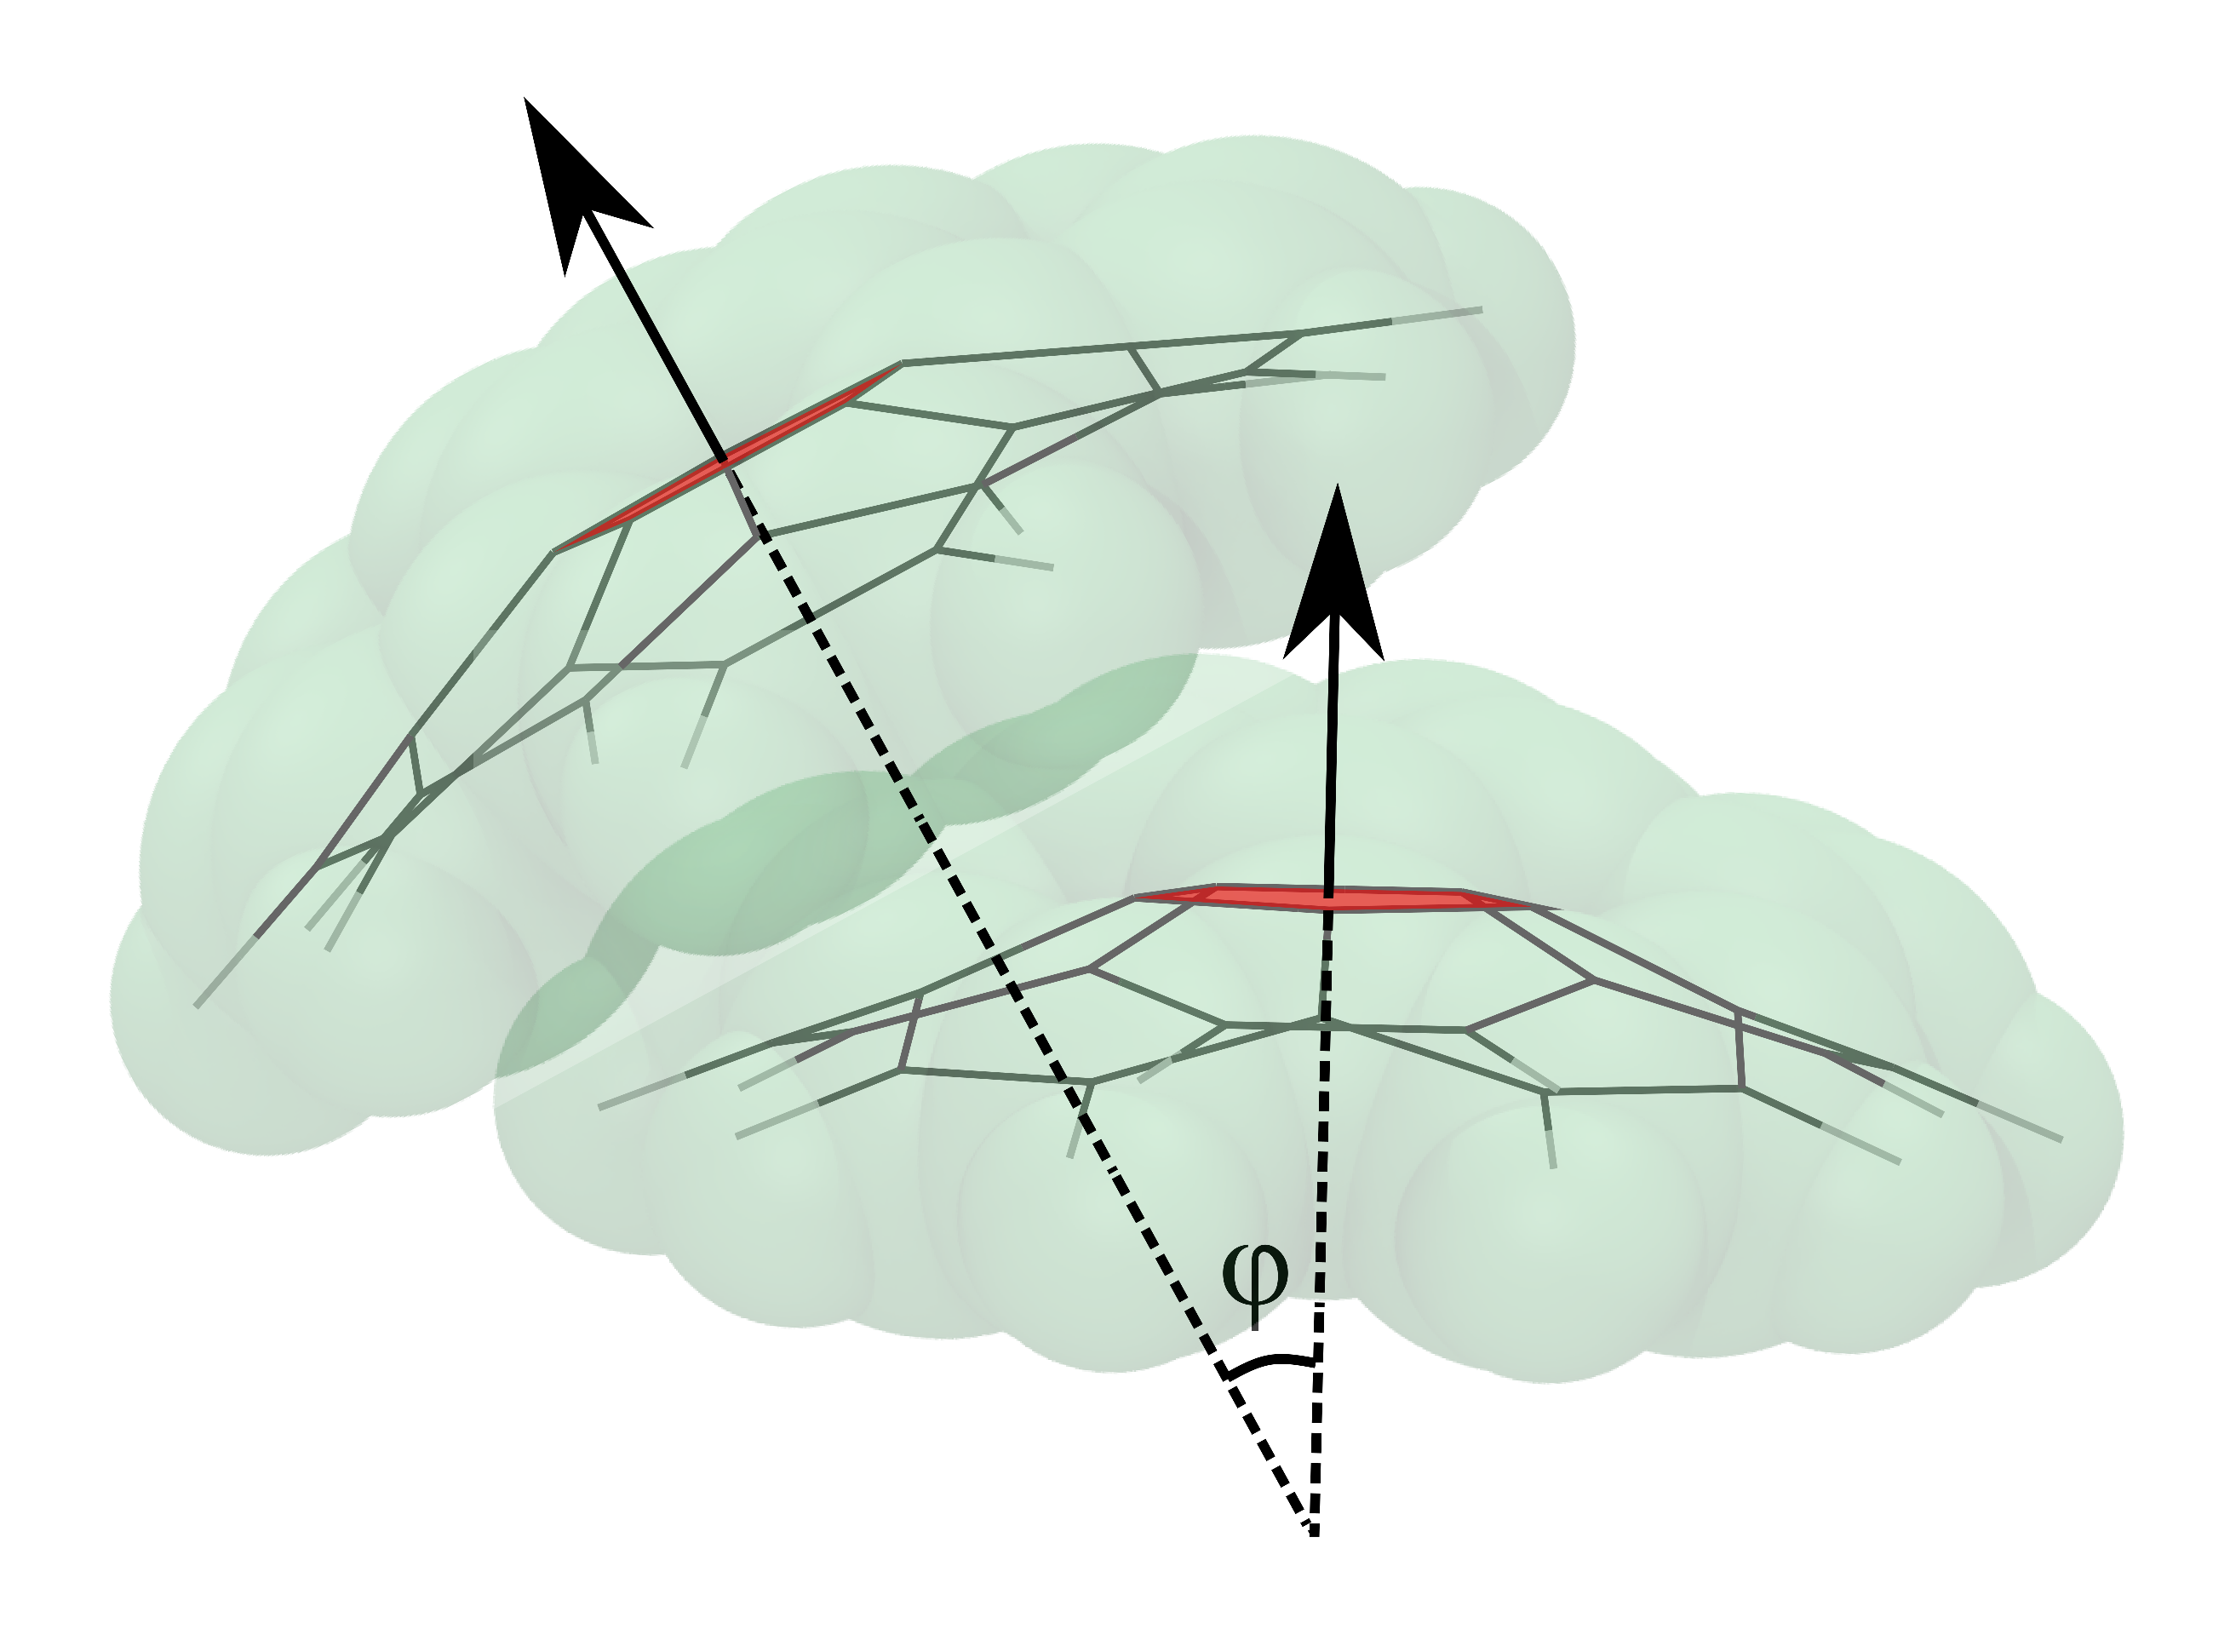
\includegraphics[width=0.25\linewidth]{Figures/alignment_angle_schematic.eps}
\caption{Schematic illustrating the calculation of the alignment angle between two neighbouring A molecules. The central pentagonal rings are highlighted in red and the alignment angle ($\varphi$) is $30^{\circ}$. \textbf{Add this to alignment angles histogram figure?}}
\label{fig:alignmentangle_schematic}
\end{figure}
%

% coordination numbers
A quantitative measure of the degree of stacking order in the molecular structures is provided through the use of coordination numbers (CNs), calculated as the number of near neighbours averaged over each molecule type. To consider only $\pi$-$\pi$ stacking interactions within this metric, values of $R$ are selected to include sandwich-type stacked interactions between molecules but exclude molecules more than one layer away. Equilibrium dimer distances provide the minimum $R$ values for each molecule type as $R_{\text{A}} = 0.4$ nm and $R_{\text{B}} = 0.5$ nm. The sensitivity of these cut-off values on calculated cluster properties is discussed in the Supplementary Information Section~XXXX. The mathematical description of the coordination number is provided in the Supplementary Information Section~\ref{secSI:raddist_CN_eqns}.

% radial distances
Radial distances are defined as the average distance between a molecule type and the cluster centre (calculated for each atom) and provide insight into the spatial partitioning of molecule types within a cluster, particularly useful for understanding the self-assembly of heterogeneous systems. Further information on the calculation of radial distances and coordination numbers is provided in the Supplementary Information Section~\ref{secSI:raddist_CN_eqns}.

%These metrics were assessed and represent the A crystal structure well (see Supplementary Information Section~\ref{secSI:corannulenecrystal} for more details).


\section{Results and Discussion}
%
\subsection{Intermolecular description of cPAHs} 
%%% The curPAHIP potential developed from corannulene energies can be used also to capture interactions between large cPAHs and mixed cPAHs %%%
%
The binding energies of cPAH dimers calculated by DFT calculations are compared to the curPAHIP intermolecular potential to assess the suitability of the latter in describing systems containing cPAHs. This is shown for four dimer types in Figure~\ref{fig:potentialDFTcurves}. The energy of the isoPAHAP potential is also included to highlight the behaviour of a PAH potential that does not include the enhanced electrostatics and dispersion due to the flexoelectric effect, and in all cases the isoPAHAP potential significantly underestimates the binding energy and overestimates the equilibrium dimer distance.
The curPAHIP potential agrees very well with the DFT and SAPT(DFT) results for the A dimer, Figure~\ref{fig:potentialDFTcurves}(a). This is expected since these \textit{ab~initio} values were used in the parameterisation of the curPAHIP potential \cite{bowal2019ion}. 
Figure~\ref{fig:potentialDFTcurves}(b) shows that the curPAHIP potential can be extended to cPAH molecules larger than A, since there is good agreement with DFT energies for the larger B molecule (within 5\% of the dispersion-corrected DFT). In contrast, the isoPAHAP gives a minimum energy value that is 31\% smaller than the DFT calculations.
The energies of heterogeneous dimers, containing one A molecule and one B molecule, are also well captured by the curPAHIP potential, as seen in Figure~\ref{fig:potentialDFTcurves}(c) and (d). Although the repulsive branch of the curPAHIP potential is slightly shifted to smaller distances than the DFT values in some cases, this is acceptable since the repulsive branch has been shown to weakly influence PAH cluster formation with the interaction well depth playing the significant role \cite{Pascazio2017}. Of note, the nested dimer with the smaller A molecule on the concave side of the larger B molecule (Figure~\ref{fig:potentialDFTcurves}(c)) shows a T-shaped type configuration. In this system the curPAHIP potential provides a slightly smaller %need to quantify? 
angle between the two molecules in the minimum energy configuration than the DFT calculation, suggesting that CH-$\pi$ interactions are weaker and $\pi$-$\pi$ overlap is favoured using the intermolecular potential.  This difference does not seem to cause a significant difference in larger systems, however, as discussed further in the alignment angle analysis. % discuss how the dimer angle is seen in the stacks (20 degrees)
%
\begin{figure}[!tbh]
\centering
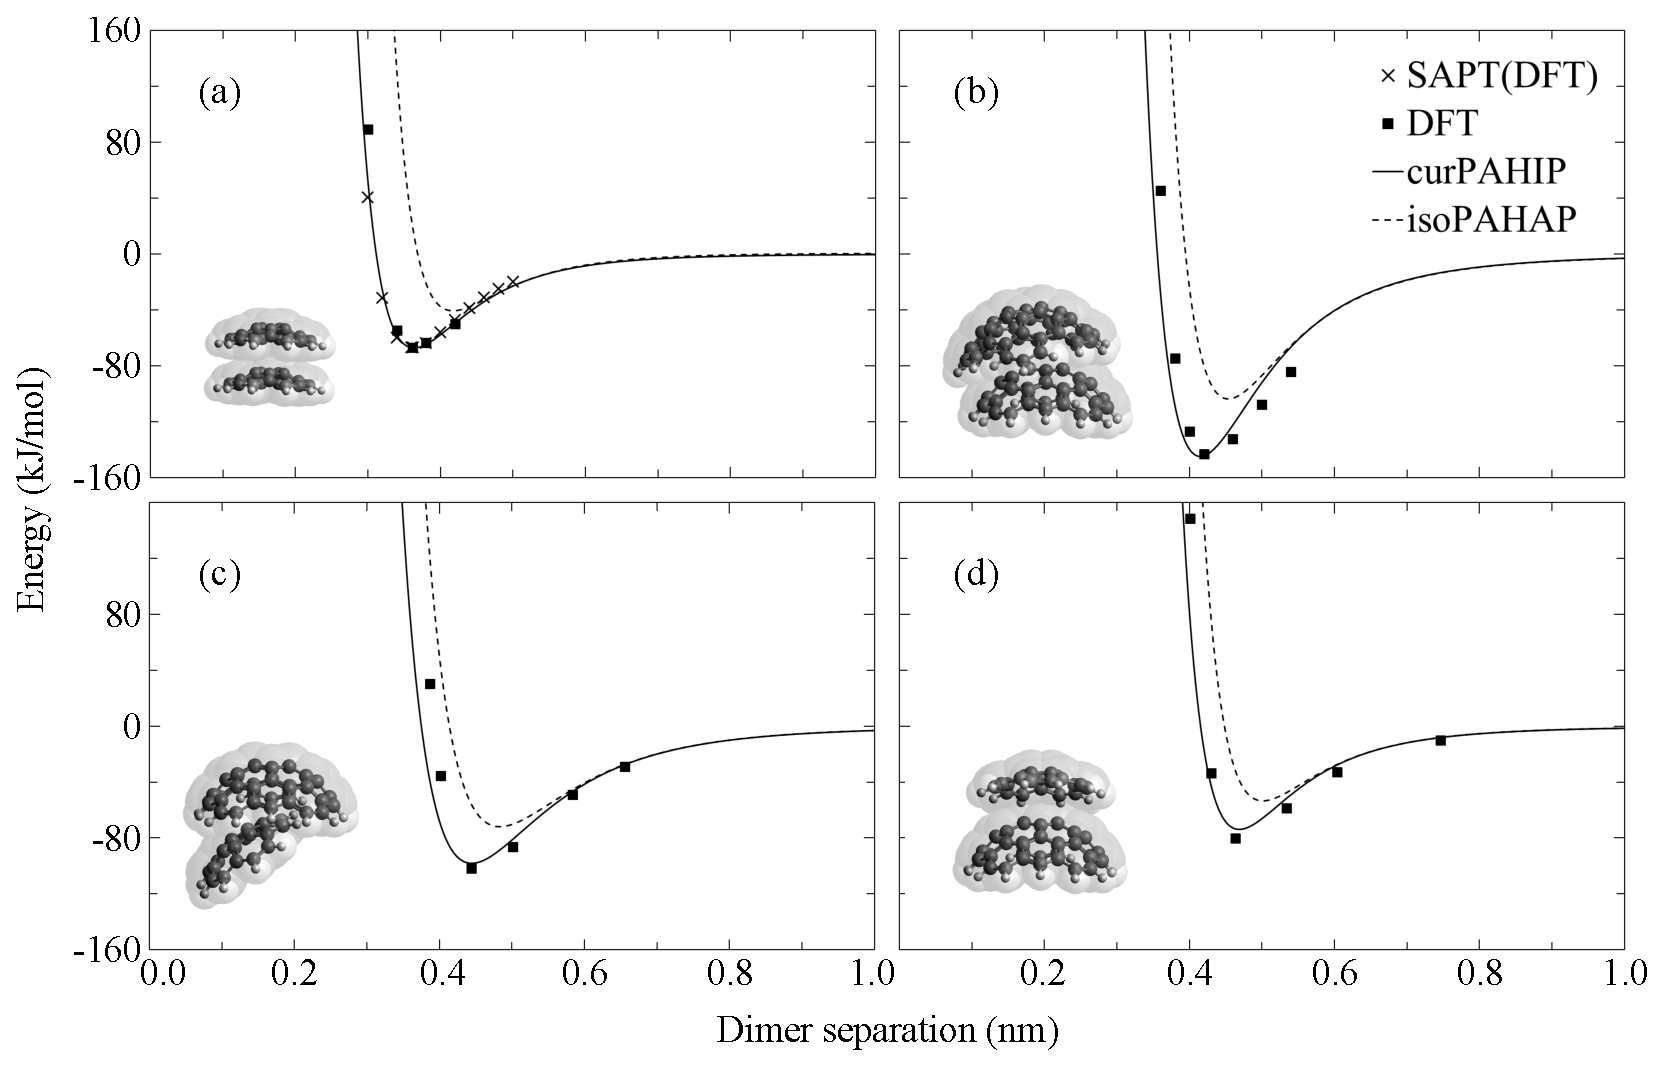
\includegraphics[width=1\linewidth]{Figures/potentialDFT_curves.eps}
\caption{Interaction energy versus separation distance for a cPAH dimers determined from SAPT(DFT) calculations \cite{Cabaleiro-Lago2018}, DFT calculations, the curPAHIP potential, and the isoPAHAP potential. The dimers are as follows: (a) two A molecules, (b) two B molecules, (c) and (d) one A and one B molecule each.}
\label{fig:potentialDFTcurves}
\end{figure}
%
%%%%%%%%% to add to discussion:
% Overall some slight differences compared to DFT results show repulsive component of curPAHIP is shifted to smaller distances (means that there might be stronger attractions at small dimer separation distances) and minimum is slightly lower energy (provides conservative case if any different (less likely to bond))
% The difference between the DFT and curPAHIP energies can be partly explained by the fact that the MD minimised monomers (used in curPAHIP assessment) are more curved than the DFT monomers. So perhaps the energies are not as low for the curPAHIP potential since the dimers are not able to reach the same small distance values without steric hindrance and repulsion coming into effect.
%
%%%%%%%%%%%%%%%%%%%%%%%%%%%%%%%%%%%%%%%%%%%%%%%%%%%%%
%%%%%%%%%%%%  HOMOGENEOUS CLUSTERS %%%%%%%%%%%%%%%%%%
%%%%%%%%%%%%%%%%%%%%%%%%%%%%%%%%%%%%%%%%%%%%%%%%%%%%%
\subsection{How do cPAHs self-assemble into a mesophase?}
% Cluster snapshots, CNs, angles show significant stacking of 2pent15ring molecules but not much for corannulene
%
%%% Cluster snapshots and macro properties (diameter, density) provided for reference %%%
Homogeneous clusters containing A or B molecules are studied to evaluate the self-assembled structures of cPAHs of different sizes and curvatures. Upon initial observation of the cluster snapshots in Figure~\ref{fig:clustersnapshots}, it is clear that these clusters self-assemble into different structural arrangements.  This will be explored further using a number of quantitative metrics. Key structural and energetic values for these clusters are given in Table~\ref{table:maintable}. Cluster diameters and densities show that both molecule types form tightly packed clusters. For example, the homogeneous A cluster densities are between 1.45 and 1.50 kg/$\text{m}^{3}$, higher than that of the A crystal structure at 1.36 kg/$\text{m}^{3}$ \cite{CORANN11unitcell} and similar to that of comparably sized fPAH clusters \cite{chen2014size}. All cluster densities decrease with increasing cluster size, although this effect is muted for cPAH clusters compared to their fPAH counterparts. 
%diameter results are as expected - the more molecules, and the larger the proportion of larger molecules, the higher the cluster diameter.
%
% Include skeletal snapshots etc?
\begin{figure}[!tbh]
\centering
\includegraphics[width=0.9\linewidth]{Figures/cluster_snapshots.eps}
\caption{Snapshots of clusters containing corannulene molecules (A), \ce{C42H14} molecules (B), and/or potassium cations (K). \textbf{Make labels larger, decrease white space.}}
\label{fig:clustersnapshots}
\end{figure}
%
%
\subsubsection{Intermolecular spacing and stacking}
%%% Intermolecular spacing: no cluster size dependence, suggests close interactions between large molecules (like dimer) compared to small molecules (which are more like crystal) %%%
The intermolecular spacing within these cPAH systems is controlled by the molecular composition of the cluster rather than its overall size.  Across all cluster sizes, A molecule spacings are around 0.60 nm, and B molecule spacings are around 0.45 nm.  The smaller spacing value for the cPAH possessing a higher curvature suggests that the molecule types configure in different arrangements that are not controlled solely by steric effects. %However both of these values are higher than the interlayer spacing of graphite (0.33 nm (ref)). 
The intermolecular spacings for dimers determined by electronic structure calculations, using the same notation as in Figure~\ref{fig:potentialDFTcurves}, are (a) 0.36 nm, (b) 0.42 nm, (c), 0.44 nm, and (d) 0.46 nm. The average spacing of B is similar to that of its sandwich dimer but the spacing of A is significantly larger. The average intermolecular spacing within a single layer of the A crystal structure characterised by X-ray crystallography is 0.57 nm, suggesting the cluster structure of A is more similar to its crystal packing than the $\pi$-$\pi$ stacking arrangement dominant in clusters of fPAH clusters.  
% intermolecular spacing of indenocorannulene molecules within crystal structures are 0.33-0.37 nm \cite{Filatov2010}. 

The intermolecular spacing of B does not change easily with the cut-off distance used indicating that the B molecules have distinct near neighbours, for example in a highly stacked configuration. In contrast, the A spacings are strongly correlated to the cut-off distance selected, suggesting that the molecules are not arranged in structured stacked layers. Intermolecular spacing values are reported for a number of cut-off distances in the Supplementary Information Section~\ref{secSI:cutoffs}.
%
% Move energy over to final column since discussed last?
\begin{table}[ht]
\centering
\caption{Cluster diameter (nm), density (kg/$m^3$), intermolecular energy (kJ/mol per molecule), average intermolecular spacing (nm), and equilibrium radial distance, $r$, of molecule A and molecule B (nm) for all clusters studied in this work.} %Properties are empirical equilibrium values, as indicated by angled braces, determined as the average over the final 3 ns of the simulation.
\label{table:maintable}
\begin{tabular}{lcccccc}
\hline
\multicolumn{1}{l}{\multirow{2}{*}{Cluster}} & \multicolumn{1}{c}{\multirow{2}{*}{Diameter}} & \multicolumn{1}{c}{\multirow{2}{*}{Density}} & \multicolumn{1}{c}{\multirow{2}{*}{Energy}} & \multicolumn{1}{c}{\multirow{2}{*}{Spacing}} & \multicolumn{1}{c}{\multirow{2}{*}{$r_{\text{A}}$}} & 
\multicolumn{1}{c}{\multirow{2}{*}{$r_{\text{B}}$}} \\ 
\multicolumn{1}{c}{} & \multicolumn{1}{c}{} & \multicolumn{1}{c}{} & \multicolumn{1}{c}{} & \multicolumn{1}{c}{} & \multicolumn{1}{c}{} & \multicolumn{1}{c}{} \\ \hline
$\text{A}_{\text{25}}$ & 2.36 & 1.50 & -75 & 0.59 &  0.91 & -- \\
$\text{A}_{\text{40}}$ & 2.77 & 1.49 & -82 & 0.59 & 1.07 & -- \\
$\text{A}_{\text{50}}$ & 3.00 & 1.47 & -84 & 0.60 & 1.14 & -- \\
$\text{A}_{\text{100}}$ & 3.79 & 1.45 & -92 & 0.59 & 1.46 & -- \\
$\text{A}_{\text{200}}$ & 4.79 & 1.45 & -97 & 0.60 & 1.85 & -- \\ \hline
$\text{B}_{\text{25}}$ & 2.96 & 1.59 & -144 & 0.44 & -- & 1.27 \\
$\text{B}_{\text{40}}$ & 3.49 & 1.55 & -152 & 0.45 & -- & 1.45 \\
$\text{B}_{\text{50}}$ & 3.76 & 1.55 & -157 & 0.45 & -- & 1.49 \\
$\text{B}_{\text{100}}$ & 4.77 & 1.52 & -165 & 0.45 & -- & 1.92 \\ \hline
$\text{A}_{\text{10}}\text{B}_{\text{30}}$ & 3.31 & 1.58 & -147 & 0.44 & 1.53 & 1.30 \\ 
$\text{A}_{\text{20}}\text{B}_{\text{20}}$ & 3.16 & 1.55 & -125 & 0.44 & 1.31 & 1.20 \\
$\text{A}_{\text{30}}\text{B}_{\text{10}}$ & 2.98 & 1.52 & -103 & 0.54 &  1.21 & 1.04 \\
$\text{A}_{\text{50}}\text{B}_{\text{50}}$ & 4.31 & 1.52 & -135 & 0.51 &  1.85 & 1.49 \\ \hline
$\text{A}_{\text{20}}\text{C}_{\text{20}}$ & 2.88 & 1.46 & -80 & 0.42 &  1.18 & 1.21 ($r_{\text{C}}$) \\ \hline
$\text{A}_{\text{40}}\text{K}_{\text{1}}$ & 2.78 & 1.49 & -88 & 0.61 &  1.06 & -- \\
$\text{A}_{\text{40}}\text{K}_{\text{2}}$ & 2.79 & 1.48 & -94 & 0.58 &  1.05 & -- \\ 
$\text{B}_{\text{40}}\text{K}_{\text{1}}$ & 3.50 & 1.54 & -149 & 0.46 &  -- & 1.35 \\ 
\end{tabular}
\end{table}
%

%%% CN results: 2pent15ring molecules are stacked, corannulene molecules aren't %%%
Coordination number values provide information on the extent of stacking interactions, which can help explain the intermolecular spacing results and elucidate internal cluster structure. The A molecule clusters showed an average CN value of $0.01 \pm 0.01$, while the B molecule clusters possess CN values of $1.48 \pm 0.09$. Therefore, as seen in the cluster snapshots, B molecules align closely with each molecule bowl inserted into the concave surface of its neighbour so that each molecule possesses on average more than one near neighbour in a stacked configuration. This is very similar to the CN values determined for fPAH clusters which arrange in a highly stacked structure \cite{bowal2018partitioning}. In contrast, A molecules do not have near neighbours within stacking distance and the molecular bowls do not pack tightly within each other. 
% Coordination number analysis will be explored in further sections.
% add results from unit cell or other literature?
% need to add CN values to table to show more homogeneous cases?  Or add to SI?
% include? "We find that the nearest neighbour coordination shells contain approximately XX molecules."
%
%Further applications: Understanding the stacking behaviour of curved PAHs is relevant to materials studies / supramolecular chemistry / crystalline organic materials because of their unique optical and conduction properties; and can also lead to using these molecules as building blocks for engineering organic crystals with desired properties.  Synthesis of curved PAH hybrids has shown that the $\pi-\pi$ interactions of these curved species can result in tight stacking in 1D columns \cite{dubceac2018self}.
% relevant to polymers of intrinsic microporosity, graphene systems, graphene quantum dots (experimental condensation structure)

\subsubsection{Alignment angles}
%%% Molecule sizes have different molecular angles %%% 
Figure~\ref{fig:alignmentangles_homo} presents histograms of the molecular alignment angles, illustrating the relative configurations of neighbouring molecules within the homogeneous clusters studied. It is immediately clear that again the two molecule sizes behave differently. The systems containing B (top row) show a single significant peak around 20$^{\circ}$.  This suggests that nearly all of the molecules interact in a tilted stacked formation, forming 1D columns in which the molecule bowls possess a face-to-face $\pi$-$\pi$ alignment. This nanostructure has significant $\pi$-$\pi$ overlaps and a small alignment angle, showing that CH-$\pi$ interactions, in which the positively charged rim of one molecule is almost perpendicular to the negative region and the bottom of the other molecule in a T-shaped configuration, are weak.  

In contrast, the systems containing A (bottom row) show a dominant peak at around 45$^{\circ}$, with smaller peaks around 130$^{\circ}$ and 170$^{\circ}$. This shows that CH-$\pi$ interactions dominate while $\pi$-$\pi$ interactions have a minor role. This structure agrees with previous work that shows A molecules do not pack with any long-range order \cite{hanson1976crystal,Petrukhina2005,kanao2018differentiating,wang2015electronic,scott1999geodesic}. It is interesting that this bulk molecular arrangement is observed even within the very small nanocluster systems examined here. The method constraints of this work highlight that this structure is not due to the rapid bowl inversion dynamics of the system but instead to the molecule size, shape, and electrostatic properties.
% multidimensional analysis shows that the local orientational order of the corannulene molecules are more complex than those of 2pent15ring.  At smaller separation/cut-off distance (< XX nm), the favoured nearest neighbour geometry is XXX (like 45deg angled? vs stacked) while at larger distances (> XX nm) it is XXX (like 90deg??).
%
\begin{figure}[!tbh]
\centering
%\includegraphics[width=0.5\linewidth]{Figures/alignment_angle_homo_draft.png}
\caption{Alignment angle distribution for homogeneous B and A clusters across different cluster sizes where $n$ indicates the number of molecules in the cluster.}
\label{fig:alignmentangles_homo}
\end{figure}
%
Both sets of homogeneous clusters present alignment angles similar to those seen in the crystal structure or minimised dimer, shown as dashed vertical lines for the A and B molecules, respectively, suggesting that these nanoclusters possess some crystal-like structure.  Although the molecule sizes show different alignment angle distributions, both cluster types show the consistent behaviour across all cluster sizes considered. Additional cluster size plots can be seen in Figures \ref{fig:alignmentangles_hetero}, \ref{figSI:alignmentangles_cutoffs}, and \ref{figSI:alignmentangles_100}.

%%% Further discussion of arrangements and comparison to literature %%%
The two molecule types show significantly different arrangements within homogeneous clusters. Strong CH-$\pi$ attractions between the molecule rims and bowl centres control the arrangement of A molecules while dipole-dipole attractions and dispersive surface interactions produce the B molecule structures. This molecule-size dependent structure is also observed within the crystal structures of cPAHs. Clusters containing B molecules form 1D polar columnar stacks with concave-to-convex $\pi$-$\pi$ bowl interactions aligned along the dipole moment vectors, like the crystal packing trends observed for molecules within the indenocorannulene family \cite{Filatov2010} and similar to that of highly curved cPAHs identified to form polar crystals with strong photoluminescence \cite{chen2014highly}. Neighbouring columnar stacks of B have opposite bowl directions and inter-stack interactions appear weak. Interestingly, the columns show significant tilting at their ends such that parallel columns curve to be nearly continuous, which is not seen in crystal structures and likely influences cluster surface properties.
% corannulene derivatives (with added rings) show significantly improved electrical conductivity compared to the parent corannulene \cite{wang2015electronic} - suggests same for B molecule
%
%%%%%%%%%%%%%%%%%%%%%%%%%%%%%%%%%%%%%%%%%%%%%%%%%%%%%
%%%%%%%%%%%%  HETEROGENEOUS CLUSTERS %%%%%%%%%%%%%%%%
%%%%%%%%%%%%%%%%%%%%%%%%%%%%%%%%%%%%%%%%%%%%%%%%%%%%%
\subsection{Do cPAHs self-assemble into core-shell nanoparticles?} 
Four clusters containing both A and B are examined to understand the self-assembly of heterogeneous cPAH clusters. The $\text{A}_{\text{10}}\text{B}_{\text{30}}$, $\text{A}_{\text{20}}\text{B}_{\text{20}}$, and  $\text{A}_{\text{30}}\text{B}_{\text{10}}$ clusters show the influence of molecular ratio, and the $\text{A}_{\text{50}}\text{B}_{\text{50}}$ cluster highlights any influences due to cluster size. Of particular interest is whether cPAHs show the same partitioning seen in fPAH systems, where the cluster core consists of the larger fPAHs and the shell contains the smaller fPAHs \cite{bowal2018partitioning}. The diameter and density values of the heterogeneous clusters containing two molecule types are consistent with simple mixing averages of the analogous homogeneous clusters, suggesting that heterogeneity does not cause a dramatic change in the overall cluster shape and packing, although further analysis needs to examine internal and molecule-specific effects.

\subsubsection{Intermolecular spacing and stacking}
%%% spacings results: spacings influenced by molecule neighbours considered %%%
The intermolecular spacings within heterogeneous clusters (Table~\ref{table:maintable}) show differences that suggest that both the molecular ratio and cluster size may play a role in the average spacing. This is investigated further in Table~\ref{table:mixedintermolecdists}, which breaks down the average results by considering the molecule-type contributions to the intermolecular spacing. This shows that the interactions between molecules of the same type maintain intermolecular spacings similar to those in the homogeneous clusters, so that the spacings between A molecules are larger than those between B molecules. The B-B spacings are similar to that of a minimised B dimer and reasonably uniform across all heterogeneous clusters.  %slightly smaller than seen for B clusters
Although the cluster size also does not influence the A-A spacing, the proportion of A plays a role. The mixed molecule interactions have similar spacings to those of the larger cPAH suggesting that the B molecule promotes the stacking behaviour of $\pi$-$\pi$ interactions with A. This is more pronounced with a higher proportion of B molecules compared to A molecules and is also cluster-size dependent. 

The differences between average spacing values for the heterogeneous clusters (for example comparing $\text{A}_{\text{20}}\text{B}_{\text{20}}$ and $\text{A}_{\text{50}}\text{B}_{\text{50}}$) are therefore observed to be largely due to the number of neighbouring A or B molecules within each cluster rather than the molecule type intermolecular spacings. % two50ann50 clusters show increased average spacing values indicating stronger contributions from A-A interactions compared to B-B interactions, even compared to the two20ann20 clusters. %two20ann20 has 22 pairs for TWO-TWO and only 4 for ANN-ANN (and 21 for TWO-ANN); two50ann50 has 24 pairs for TWO-TWO and 26 for ANN-ANN (and 23 for TWO-ANN).
In this way the cluster spacing averages provide an indication of which molecule pairings are most prevalent. %- what type of stacking is most dominant. 
% include proportion / percentage values for each interaction type from number of pairs in each case? 
%
\begin{table}[thb]
\centering
\caption{Intermolecular spacings within heterogeneous clusters, considering average distances between molecule types A and B.}
\label{table:mixedintermolecdists}
\begin{tabular}{lccc}
\hline
Cluster & B-B & B-A & A-A \\ \hline
$\text{A}_{\text{10}}\text{B}_{\text{30}}$ & 0.43 & 0.43 & 0.53 \\
$\text{A}_{\text{20}}\text{B}_{\text{20}}$ & 0.43 & 0.41 & 0.61 \\
$\text{A}_{\text{30}}\text{B}_{\text{10}}$ & 0.44 & 0.48 & 0.58 \\
$\text{A}_{\text{50}}\text{B}_{\text{50}}$ & 0.44 & 0.47 & 0.60 \\
\hline
\end{tabular}
\end{table}
%

%%% CN results: addition of 2pent15ring into corannulene clusters increases stacking %%%
To clearly examine the influence of compositional heterogeneity, coordination number values are compared across different clusters all containing 40 cPAH molecules, shown in Figure~\ref{fig:coordination_numbers}. The molecule-specific CN values within these heterogeneous clusters aligns with those calculated for homogeneous clusters. The B molecules within all clusters have CN values above 1, indicating that on average these molecules have more than one near neighbour in a stacked arrangement. In contrast, all A molecules have CN values significantly below 1, which shows that these molecules do not arrange in close stacks.  
% For these 40 molecule clusters, the CN values are: ann < 10t30a(a) < 2020(a) < 30t10a(a) < 10t30a(t) < 20/20(t)=two < 30t10a(t).  
The CN values for both molecule types follow the trend $\text{A}_{\text{40}} < \text{A}_{\text{30}}\text{B}_{\text{10}} < \text{A}_{\text{20}}\text{B}_{\text{20}} < \text{A}_{\text{10}}\text{B}_{\text{30}}$, which shows that the addition of B molecules into A clusters increases the CN values.
%
\begin{figure}[!bth]
\centering
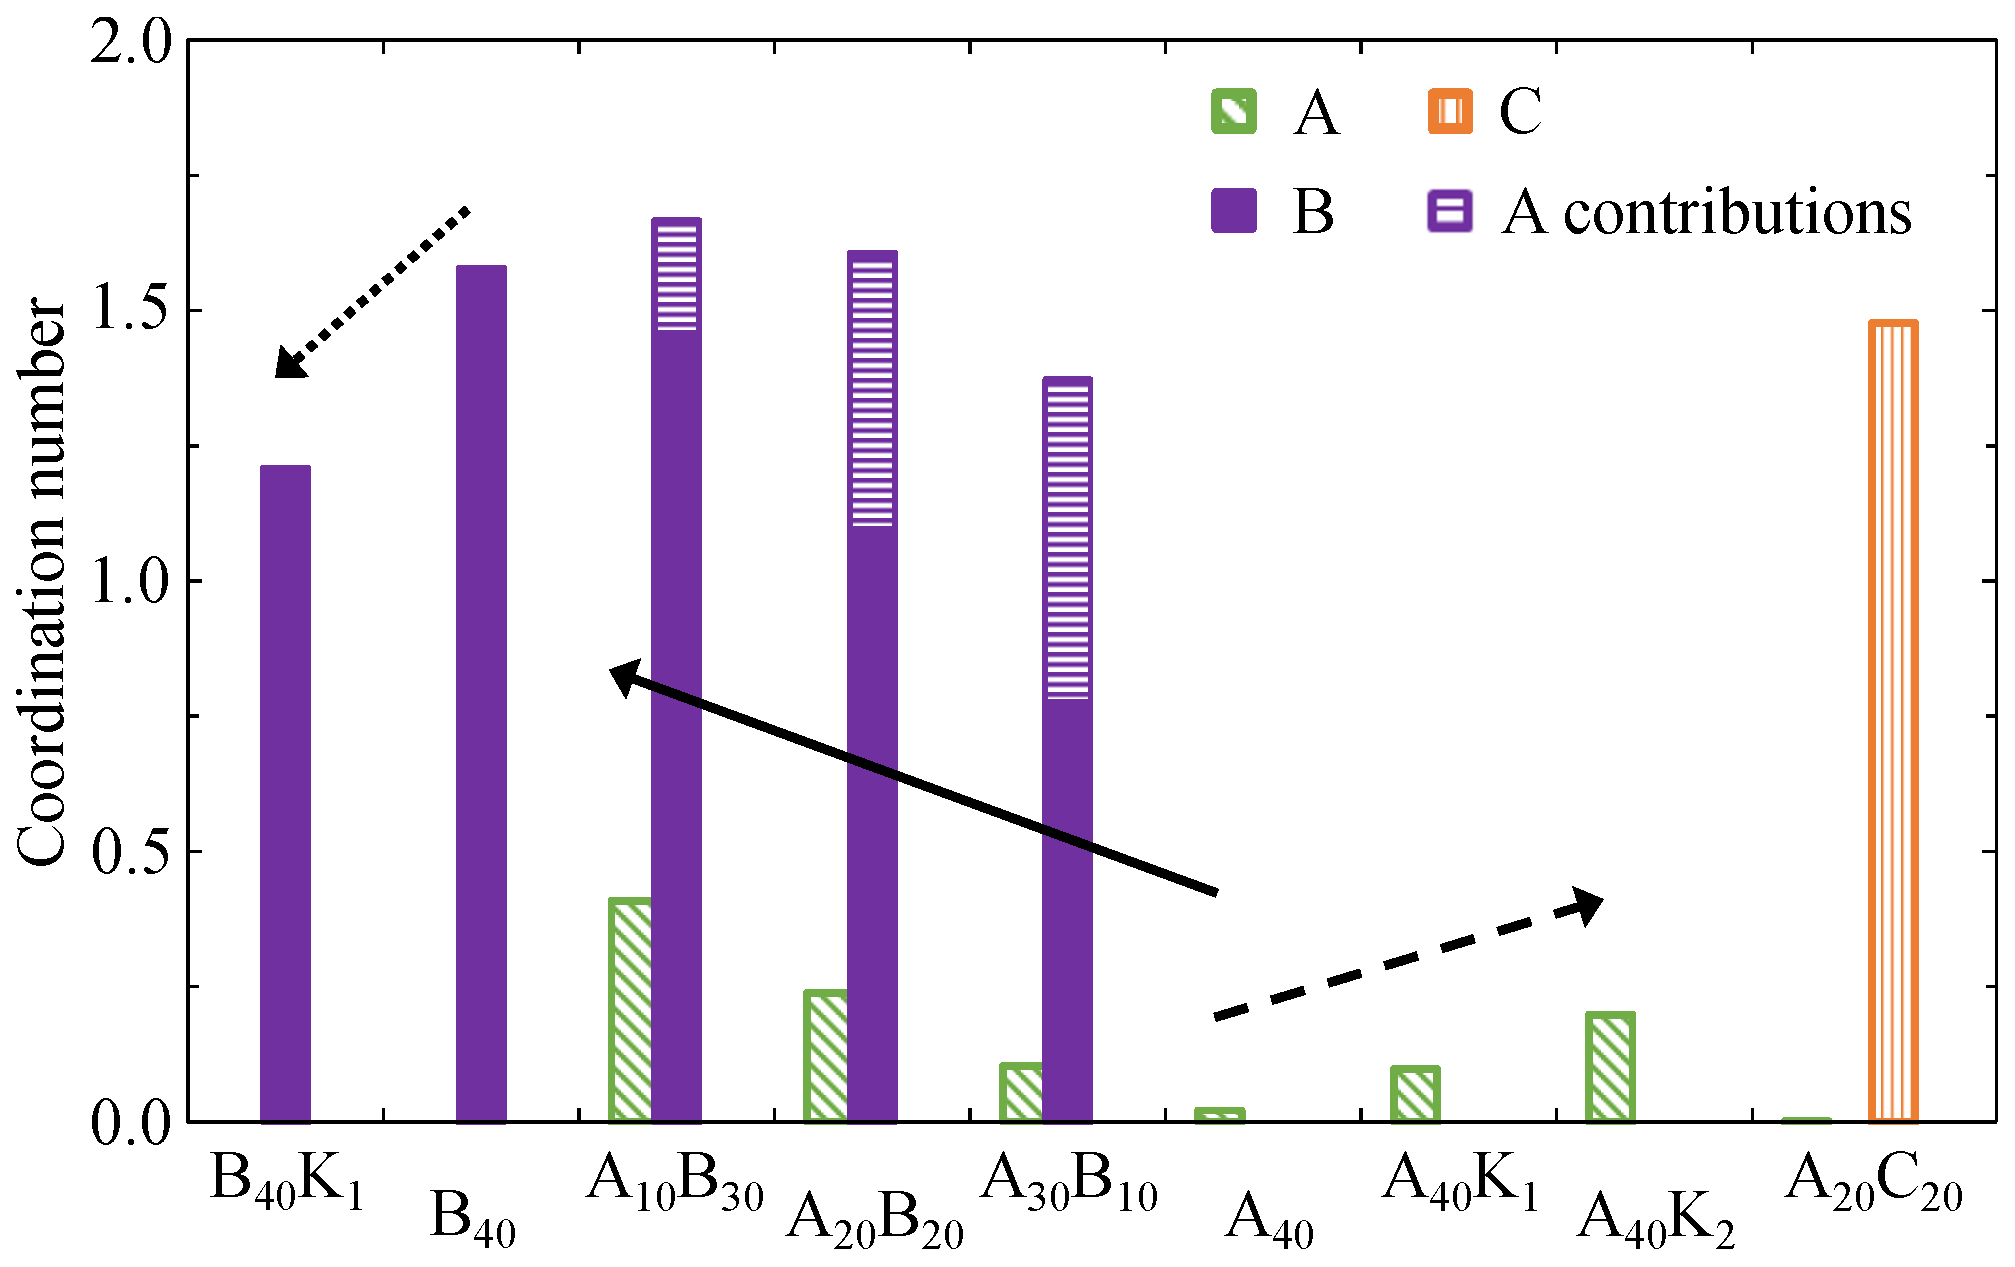
\includegraphics[width=0.8\linewidth]{Figures/CN_bar_chart_updated.eps}
\caption{Coordination number values across clusters containing 40 molecules.}
\label{fig:coordination_numbers}
\end{figure}
%
% perhaps include cluster snapshots with ribbons to show stacking more clearly?  As insets in bar chart?

Further analysis is conducted to determine which molecule types are present as near neighbours within heterogeneous systems. The CN values of A molecules have no contribution from A molecules, so all A stacking interactions come from neighbouring B molecules. The B molecule stacking interactions come predominantly from other B molecules, however a proportion of the interactions are with A molecules in proportion to the molecular ratios within the cluster, shown as insets with horizontal lines in the B columns of Fig \ref{fig:coordination_numbers}.
% Contribution of B stacking that came from interactions with A are: two30ann10 12\%, two20ann20 32\%, two10ann30 43\% - goes up with molecule type ratios.
%
% Cluster size does not influence structure but molecule size does (seen in CN and intermolecular spacing values).

\subsubsection{Alignment angles}
%%% Influenced by mixing and addition of cation(s) %%%
% mixed 50/50 - compare to homo systems, increasing cluster size
%Next we examined the influence of molecule size mixing on the alignment angle distribution.  
Figure~\ref{fig:alignmentangles_hetero} shows the following clusters: (a) homogeneous B, (b) homogeneous A, (c) heterogeneous containing 50\% of each molecule type. The individual molecule alignment angle distributions retain many of their features as in the homogeneous clusters with the majority of the B molecules around 20$^{\circ}$, and many of the A molecules around 45$^{\circ}$.  However, there is a distinct second peak around 45$^{\circ}$ suggesting a deviation from the stacked columns in the homogeneous B clusters. The A peaks in the heterogeneous cluster are also slightly shifted, with the peak at 45$^{\circ}$ spread out towards 0$^{\circ}$ and the peak around 120$^{\circ}$ relatively insignificant.
The angle peaks align reasonably with those seen in the A crystal structure and B dimer. %(esp for the 100 molecule cluster)
%say something about corannulene molecules being sandwiched between larger ones and how this influences the angles...
%
\begin{figure}[!tbh]
\centering
%\includegraphics[width=0.7\linewidth]{Figures/alignment_angle_hetero_draft.png}
\caption{Alignment angle distributions for heterogeneous B and A clusters containing 40 molecules. $n$ indicates the number of molecules of each type in the cluster. \textbf{To do: Need to clean up figure, label (a), (b), (c), etc}}
\label{fig:alignmentangles_hetero}
\end{figure}
%

% mixed mixed - compare to homo and other mixed systems
The influence of molecular ratio in the heterogeneous clusters is shown in clusters of the same size containing 75\% A Figure~\ref{fig:alignmentangles_hetero} (d) or 75\% B Figure~\ref{fig:alignmentangles_hetero} (e). These clusters show similar behaviour to the homogeneous and equi-ratioed heterogeneous clusters.  Interestingly, the second peak of B molecules at around 45$^{\circ}$ is more pronounced in the system containing more B molecules, suggesting that this is found in the molecules that connect stacks of B molecules.  Also in the cluster with fewer A molecules, there are increased interactions similar to B at 20$^{\circ}$. This indicates that the A molecules are stacking in a similar fashion to B, which can be seen in the cluster snapshot (Figure~\ref{fig:clustersnapshots}) where the A molecules predominantly interact individually at the ends of B molecule stacks, fitting in similarly in the concave or convex surfaces.

\subsubsection{Radial distances}
%%% Core-shell type partitioning of molecule sizes - not as distinct as fPAHs and not dependent on cluster size or molecular ratio %%%
Average radial distances between each molecule type and the cluster centre are calculated to provide an indication of the molecule-type positioning within each cluster, tabulated in  Table~\ref{table:maintable}. For the homogeneous cases, the two molecule types show similar equilibrium radial distances at 75-85\% of the total cluster radius. However, in all clusters containing two molecule types the A molecules possess larger radial distances (located within 80-90\% of the total cluster radius) than the B molecule (70-80\% of the cluster radius). This is indicative of a core-shell structure in which the larger molecules reside in the cluster core, as seen in the fPAH clusters \cite{bowal2018partitioning}.
% perhaps take out tabulated values and just show within Figure as dashed lines - can include radial distances in SI table.

Although the average radial distances show this core-shell partitioning of molecule sizes, examining the equilibrium distribution of radial distances shows that this radial separation is less distinct for clusters containing cPAHs compared to similar fPAH clusters. Figure~\ref{fig:radialdists_atomic} shows that there is significant mixing of the molecule types within the cPAH clusters, regardless of cluster size or molecular ratio.

%
\begin{figure}[!tbh]
\centering
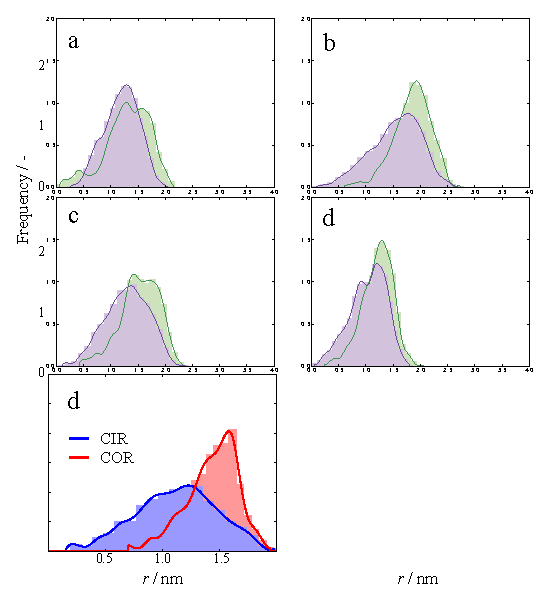
\includegraphics[width=0.8\linewidth]{Figures/radii_histograms_aa.eps}
\caption{Normalised atomic radial distance distributions for heterogeneous PAH clusters. The fPAH cluster $\text{C}_{\text{16}}\text{D}_{\text{16}}$ is obtained from \citet{bowal2018partitioning}. Molecule D refers to circumcoronene (\ce{C54H18}).}
\label{fig:radialdists_atomic}
\end{figure}
%

\subsubsection{cPAHs and fPAHs}
\textbf{TO WRITE... (incorporate into other sections or keep separate?)}
- show that cPAHs and fPAHs are immiscible 
- relevant to formation / nature of janus particles, for example ones that are polar on one side
- Also indicates that there must be bonds in soot particles because don’t see partitioning between curved and planar molecules experimentally!
- Soot structures seen experimentally do not form through self-assembly
- explain potential used and explain differences - show both cases in the SI

We conducted preliminary work assessing the properties of clusters containing cPAHs and fPAHs (corannulene and coronene). The results showed a distinct partitioning of the molecule types in a janus configuration. This can be clearly linked to stronger interactions between similar molecules compared to the mixed molecule interactions, which are hindered by sterics and do not experience any enhancement in electrostatic interactions (in a non-polarisable potential description).

Compare with experimental morphologies (do we see sections of curved/planar together?)
Relate these clusters and their properties to experimental structures (potential implications for synthesis, potential applications, etc).

Include comparison/discussion with other modelling study of fPAHs/cPAHs/fPAHs+cPAHs in \cite{zhang2020molecular}.

- Add radial distances, snapshots

- bkgd: corannulene soluble in common organic solvent (see lit review doc)

\subsubsection{Energies}
The intermolecular energies as a function of cluster mass are shown in Figure~\ref{fig:energies}.  The energies are shown per atom in the system, in order to facilitate direct comparison between systems of different cluster and molecule sizes. It is clear that in all cases the energy decreases with cluster mass, for clusters containing curved or planar PAHs. Homogeneous clusters containing planar PAHs, taken from \citet{chen2014size,chen2015solid}, show relatively consistent energy trends across molecule sizes from pyrene to circumcoronene (all coloured the same here to allow for ease in reading), with heterogeneous clusters, taken from \citet{bowal2018partitioning}, generally at lower energy values. Clusters containing the cPAH B show energies similar to those of heterogeneous fPAH clusters, while clusters containing the cPAH A have lower energies.
The effect of heterogeneity in cPAH clusters shows a distinct effect of molecular ratio: an increased proportion of B in the cluster decreases the energy. At 50\%/50\% molecule type partitioning, the heterogeneous cluster reflects that of a homogeneous A cluster (across cluster size). However, when the cluster contains only 25\% B, the cluster has significantly higher energy and inversely with 75\% B, the cluster's energy decreases significantly.  This suggests that the presence of B molecules increases cluster stability if above 50\% composition.

These trends agree with the CN value trends observed previously and highlights that lower energy heterogeneous clusters have higher CN values (more ordering). %- except A, which has very low CN values. 
Both the CN and energy values suggest that B clusters with some added (<50\%) A are the most stacked and stable.

The energy of a cluster containing both curved and planar PAHs has an energy similar to that of homogeneous coronene clusters, showing that in these cases (not including some advanced interactions such as induced dipoles, 50/50\% split, very similar sizes so less cooperative perhaps) the mixing of molecule types does not enhance the interaction energy - it remains similar to that of the weaker component.  Further work to thoroughly develop/assess a fPAH-cPAH intermolecular potential and test the effect of molecular composition should be done to further explore the possible synergistic effects of clusters containing cPAHs and fPAHs.

%%%%%%%%%%%%%%%%%%%%%%%%%%%%%%%%%%%%%%%%%%%%%%%%%%%%%
%%%%%%%%%%%% ION-CONTAINING CLUSTERS %%%%%%%%%%%%%%%%
%%%%%%%%%%%%%%%%%%%%%%%%%%%%%%%%%%%%%%%%%%%%%%%%%%%%%
\subsection{How do cPAHs self-assemble around ions?}
%%% ions change the structure of cPAH clusters different depending on molecule size %%%
An additional exploration into the influence of heterogeneity with cations is conducted by considering clusters containing 40 molecules (A or B) and one or two potassium ions.  These systems can be directly compared to homogeneous systems of the same size. Potassium ions are selected because they are known to interact with cPAHs in systems of interest (refs combustion/production) and because the intermolecular interactions between this cation and cPAHs have already been parameterised with the curPAHIP potential \cite{bowal2019ion}. As seen in Table~\ref{table:maintable},
the inclusion of ion(s) within the cPAH clusters appears to increase the cluster diameter, and thus decrease the cluster density, slightly.

\textbf{To Do: include discussion/comparison to results of solvation shells of fPAHs around ion(s) - from \cite{bowal2019ion,bartolomei2019aggregation}.}

\subsubsection{Intermolecular spacing and stacking}
Intermolecular spacing values also change slightly with the addition of a cation(s). The B cluster experiences a small increase in the spacing, while the A clusters show an increase and decrease in the spacing values depending on the number of cations present. This suggests that the cation has an effect on molecular arrangement, although in opposite ways depending on the constituent cPAH size. % differences maybe not big enough to make these statements?!  Shorten this paragraph (already mostly combined below)

The CN values for ion-containing clusters complement the intermolecular spacing results. The B cluster CN value decreases with the addition of \ce{K+}, suggesting a disruption of the highly stacked ordering and matches an increased intermolecular spacing. Conversely, the A clusters show some increased ordering with higher CN values and also decreased average spacing. This effect increases with the addition of a second cation, although the CN values are still significantly lower than those of the B clusters.

\subsubsection{Radial distances} % take out this section??  First sentence can be added to earlier section.
The addition of a potassium cation(s) also results in slightly %(2-3\%)
decreased radial distances for both molecule types, so that average molecular distance values are around 75\% of the total cluster radius. Radial distance histograms show that introducing \ce{K+} into cPAH clusters produces an increase of cPAH molecules with very small radial distance values, suggesting that the ion(s) promotes an increased molecular ordering at/around the cluster centre. This is more marked for the B cluster case than A. 
The radial position of the ion(s) within the cluster does not correspond to a clear grouping/structure of cPAH molecules. % need to unpack this more - look at expected shell around ion
% add or reference corresponding figure(s)?
%note that this is visible in homo cPAH molecular radial distance histograms not show... see log notes.  Perhaps include these plots - can overlay histograms to show effect.  Can show ion position(s) with dashed lines in these plots.  And this could segue into talking about how the ion(s) influence the molecular structure around them...
Therefore, although the presence of an ion(s) causes more cPAH molecules to order around the cluster centre, this does effect seems to be very local and the total cluster shape/size is not changed very much. The ion(s) only influence a single shell of molecules and this has only an indirect effect on the rest of the molecules. % ???
The average radial distance decreases with the addition of a second cation. %% not significant enough??
This suggests that the cation influence is additive, although further work needs to be done to assess when this trend reaches a saturation level (maximum effect) or perhaps has cancelling or negative effects. 

\subsubsection{Alignment angles}
The alignment angle distribution broadens for the B system with the addition of a cation (Figure~\ref{fig:alignmentangles_hetero}(f)), with additional angles present at approximately 55$^{\circ}$ and 135$^{\circ}$.
The A clusters containing \ce{K+} are also different than the homogeneous case, with a broadening and splitting of the 45$^{\circ}$ peak, increase in the 120$^{\circ}$ peak, and disappearance of high (around 170$^{\circ}$) angles. This shows that the addition of a cation disrupts the stacked structure otherwise seen in homogeneous or heterogeneous clusters containing B molecules. This can also be seen in the cluster snapshots in Figure~\ref{fig:clustersnapshots}, where the molecules are clustered with their electron-rich convex surfaces facing the cation but a lack of clear structure beyond this first layer of molecules surrounding the cation.
The addition of cation(s) show XXXXX alignment angle distribution that indicates the loss of regular local structure.
% It is interesting to note that the number of neighbouring molecules within the cut-off distance decreased for 2pent15ring molecule systems with the addition of a potassium cation. (this is seen in comparing cut-off distances behaviour) - is this still true after recalculating?

\subsubsection{Energies}
%%% ann clusters have lower mass-weighted energy than 2pent15ring, addition of some corannulene decreases energy (50/50 gives same as ann), fPAHs have higher energies %%%


The presence of cation(s) in the cluster has opposite effects on clusters containing the two molecule types: B clusters with \ce{K+} show an increased energy, while clusters with A molecules containing \ce{K+} showed a decreased energy in proportion with the number of ions.  These differences are shown by black arrows in Figure~\ref{fig:energies}. This suggests that the ion influences molecular interactions and cluster structure in different ways depending on the molecule size. These trends agree with the CN value trends observed previously... 

%The reason for and structural contribution/manifestation of these energy differences will be explored further in the subsequent sections.
%
\begin{figure}[!tbh]
\centering
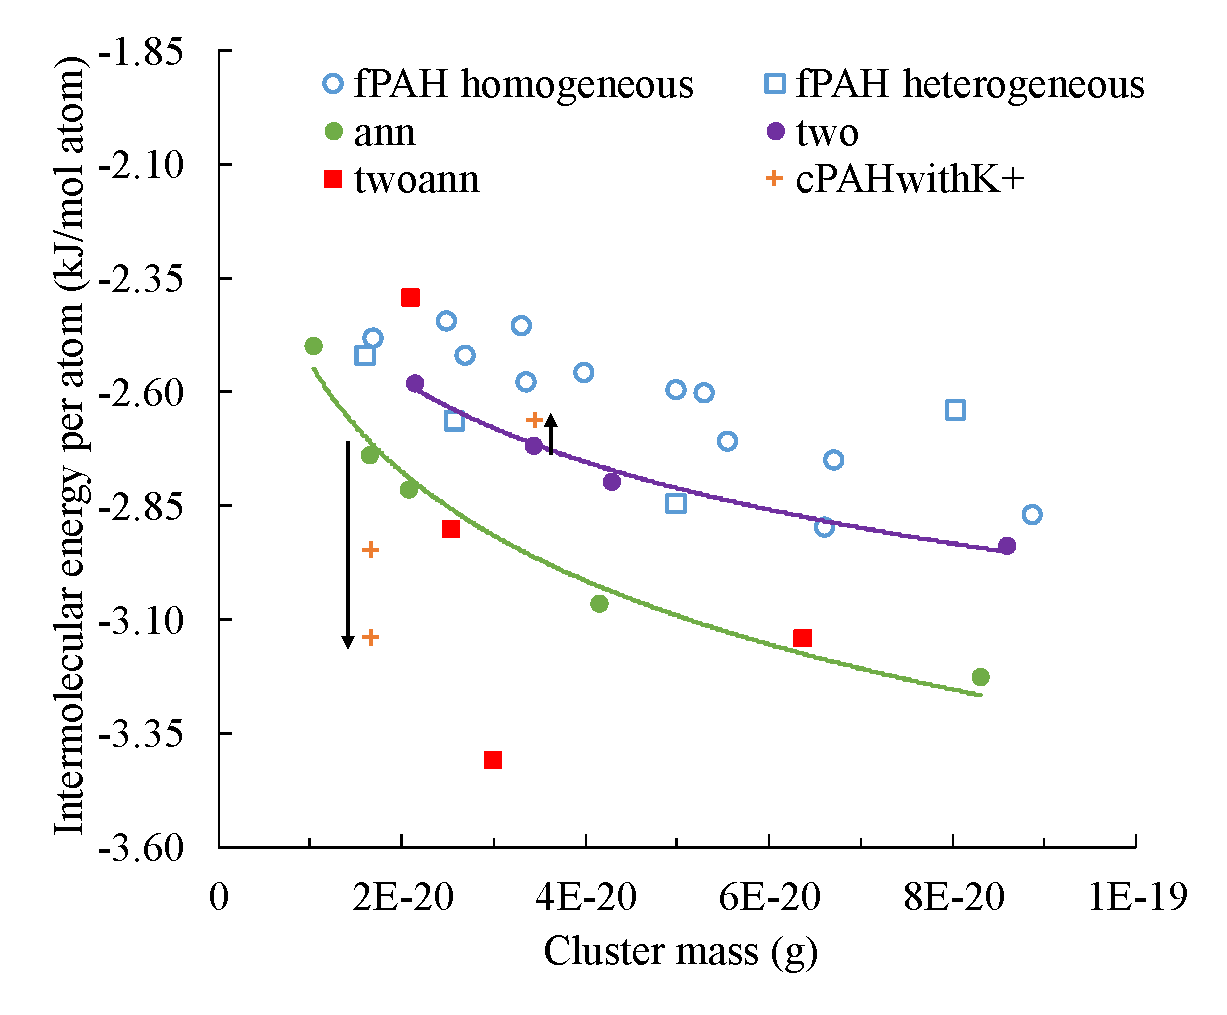
\includegraphics[width=0.5\linewidth]{Figures/energies.eps}
\caption{Intermolecular energy per atom versus cluster mass for all clusters considered in this work. Lines are drawn for the cPAH homogeneous clusters to guide the eye and black arrows show the energy changes caused by the addition of a cation(s). The subscript y is used to denote an unspecified number of molecules in order to consider multiple clusters.}
\label{fig:energies}
\end{figure}
%

%\section{Discussion}
%Further discussion highlighting main similarities and differences between cluster types as well as key findings.
%
%\subsection{Temperature effects}
%include radial distance histograms with high temperature insets?

\section{Conclusions}
\textbf{TO WRITE...}
- Curved carbons have great promise in many applications such as understanding particulates, novel nanocarbon materials, sensors
- These results provide a first detailed exploration of the nanostructure of clusters containing cPAHs and cation(s), and further work should examine the influence of ion type (cation vs anion), size, and number.
- The molecular arrangements of these homogeneous clusters show that these cPAH cluster systems behave similarly to the crystal structures of comparable cPAHs.
- Future work:
- Interactions between curved aromatic molecules containing heteroatoms, such as oxygen, show increased dimer interactions that provide further electrostatic stabilisation \cite{Cabaleiro-Lago2018}.  Future work should consider the presence of additional atoms...

\section*{Acknowledgements}
This work used the ARCHER UK National Supercomputing Service (\url{http://www.archer.ac.uk}).
K.B. is grateful to the Cambridge Trust and King's College, Cambridge for their financial support.
This project is also supported by the National Research Foundation (NRF), Prime Minister's Office, Singapore under its Campus for Research Excellence and Technological Enterprise (CREATE) programme.
